% Copyright (C) 2010 Thomas L. Kula
% All Rights Reserved
%
% See the file LICENSE for license terms.
\documentclass[12pt]{article}
\usepackage{graphicx}
\usepackage{rotating}
\usepackage{fix-cm}
\setlength{\paperwidth}{5.5in}
\setlength{\paperheight}{8.5in}
\setlength{\textheight}{7.45in}
\setlength{\topmargin}{-1.0in}
\setlength{\oddsidemargin}{-0.5in}
\setlength{\evensidemargin}{-0.5in}
\setlength{\textwidth}{4.0in}
\setlength{\parindent}{0in}
\setlength{\parskip}{3mm}
\usepackage[print]{booklet} \nofiles
\source{\magstep0}{5.5in}{8.5in}
\target{\magstep0}{11in}{8.5in}
\setpdftargetpages
\pagestyle{empty}
\begin{document}


\begin{center}
{\fontsize{36}{48}\selectfont \textsc{Haiku a Day }}
\end{center}

\vspace*{3.5cm}

{\fontsize{26}{52}\selectfont 

With doors open wide

I enjoy some good coffee

Watching the world pass

}

\vspace*{5.0cm}
\begin{center}
{\large{Issue 57: March 2010}} \\[5mm]
{\fontsize{8}{8}\selectfont  \textsc{ St. Joshua Norton Press }} \\[1mm]
{\fontsize{6}{6}\selectfont Mathom House in Midtown \textbar The People's Republic of Ames }
\end{center}


\newpage

The only thing that could make a pleasant day at the coffee shop better
is hearing the Flaming Lips album {\em The Soft Bulletin}. Today is a
good day.


--- Thomas

http://kula.tproa.net/had/ \\
kula@tproa.net

Download this and previous HADs at the website, so you can
print out your own (DIY, yeah!) or if you want me to send
you one, send me your address, and maybe a stamp if you
are feeling nice. Or send me something you've made ---
trades always appreciated, postcards are nice too.

\vspace*{2cm}

1 March 2010

Oh soup, I sing out \\
The joy you bring, exquisite \\
Fills my heart with glee

2 March 2010

Brain a whirlwind \\
Bringing order from chaos \\
Wind stops, brain cools down

3 March 2010

Stare into the night \\
Behold the stars high above \\
Feel small where you are

\newpage

4 March 2010

Beware peer pressure \\
That lunch you brought in to work \\
Pales at their onslaught

5 March 2010

The old Friday role \\
Having caffeine and coding \\
Meeting up with friends

6 March 2010

Pleasantly full day \\
Going all over the place \\
Doing many things

7 March 2010

The winter basement \\
Pales against the spring outdoors \\
Polo moves outside

8 March 2010

Glorious day erupts \\
An early spring issues forth \\
Is winter now dead?

9 March 2010

Infinitely small \\
A point strung infinitely \\
A line, length from void

10 March 2010

These forms make no sense \\
Sitting in the waiting room \\
Health care confuses

\newpage

11 March 2010

Go away snow, flee \\
Your cover is not wanted \\
Let the green return

12 March 2010

Bowling computer \\
You record our score, poorly \\
Have we confused you?

13 March 2010

Mailing us to say \\
You will soon be mailing us \\
Census makes no sense

14 March 2010

Total exhaustion \\
All I can do is sit there \\
Finally I move

15 March 2010

With a renewed shine \\
The sun illuminates us \\
Dark at lunch, light now

16 March 2010

I hear the city \\
Wafting through open windows \\
Moving the curtains

17 March 2010

Going for a walk \\
As the sun slowly sinking \\
Gives way to the night

\newpage

18 March 2010

A drunken asshole \\
With a squeal and loud crash \\
Hits the neighbor's car

19 March 2010

The first green budding \\
In the hedge by a sidewalk \\
I walk by, smile

20 March 2010

Inside a book store \\
Pleasant hours can be spent \\
Good finds your reward

21 March 2010

Breakfast cravings rise \\
Leading to omlettes at night \\
Inverting is fun

22 March 2010

Woken up at 1 \\
Leads to a long tired day \\
Going home early

23 March 2010

Drawing to a close \\
The evening turns to pastels \\
The day fades away

24 March 2010

I still want a kite \\
And a day spent in the park \\
Instead of working

\newpage

25 March 2010

Invading my head \\
Some sort of rude snot monster \\
Here without asking

26 March 2010

A vain search reveals \\
Nothing at the pharmacy \\
To erase this snot

27 March 2010

The KDC fails \\
With abandon, ruthless dies \\
Restoration weird

28 March 2010

Ruthless is happy \\
Albeit hacked together \\
Next weekend will fix

29 March 2010

Dazed and confused I \\
Awake for another day \\
Will today make sense?

30 March 2010

A ladder reaching \\
Edging high into the sky \\
Stands grounded in Earth

31 March 2010

The sun, glorious \\
Reigning over the noon sky \\
Lighting all the world


\newpage

\begin{center}
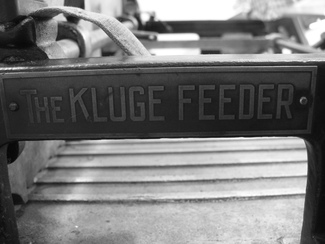
\includegraphics{vgkids-open-house.jpg} \\[1cm]

VG Kids New Production Facility Open House \\
\small{{\tt http://kula.tproa.net/photos/2010/20100319-vgkids-open-house/ }}

\end{center}

\newpage

\thispagestyle{empty}
\vspace*{14cm}
\begin{sideways}
\Large{Thomas L. Kula}
\end{sideways}
\begin{sideways}
\Large{PO Box 980461}
\end{sideways}
\begin{sideways}
\Large{Ypsilanti MI 48198}
\end{sideways}


\end{document}


